%! TeX program = lualatex
\documentclass[twoside, a4paper, 12pt]{book}

\title{Geometryczna Teoria Grup}
\author{\color{subtext1}Weronika Jakimowicz}
\date{Zima 2024/25}

% \usepackage[T1]{fontenc}

\usepackage{fontspec}
\usepackage[default]{cantarell}

\usepackage[nolessnomore,noequal,noparenthesis,nospecials,noplusnominus,noexclam,italic]{mathastext}

\usepackage{amsfonts}
\usepackage{amsmath}
\usepackage{amssymb}

\usepackage{array}


\usepackage{ntheorem}

\theorembodyfont{\normalfont}
\theoremseparator{.\hspace{0.5em}}
\theorempreskip{}
\theorempostskip{}

\theorempostwork{\vspace*{4mm}}

\newtheorem{zadanie}{Zadanie}


\pagestyle{empty}

\usepackage{tikz}
\usetikzlibrary{calc}

\usepackage[a4paper, total={170mm, 237mm}]{geometry}

\usepackage{enumitem}

\newcommand{\rozwiazanie}[1]{\slshape }%#1}

\makeatletter
\def\@maketitle{
  \begin{center}
    {\LARGE\@title}
    \medskip 

    \large\@author
  \end{center}
}
\makeatother


\usepackage[dates, pl]{../../../template}

\usepackage{halloweenmath}

\begin{document}
\frontmatter 
\maketitle
\thispagestyle{empty}
\setcounter{page}{0}

\tableofcontents
\mainmatter

\pagestyle{fancy}
  
\section{02.10.2024}{Grafy Cayleya}

\subsection{Metryka słów}

\begin{definition}{metryka słów}{}
  Niech $G$ będzie grupą, a $S$ dowolnym układem jej generatorów. Wówczas dla dowolnych $g_1,g_2\in G$ \buff{odległość między nimi w metryce słów} definiujemy jako
$$ds(g_1, g_2)=\min\{n\;:\;g_2=g_1s_1,...,s_n,\;s_i\in S\cup S^{-1}\},$$
gdzie $S^{-1}=\{g^{-1}\;:\;g\in S\}$.
\end{definition}

Metryka słów jest 
\begin{enumerate}
  \item skończona
  \item symetryczna (z definicji generatorów)
  \item \hl{lewo-niezmiennicza}, czyli $(\forall\;\gamma\in G)\;ds(\gamma g_1,\gamma g_2)=ds(g_1, g_2)$
\end{enumerate}
Ostatnia własność oznacza, że $G$ działa na sobie jako na przestrzeni metrycznej przez izometrie.

Gromov chce patrzeć na dyskretne przestrzenie metryczne, jakimi są grupy z metryką słów, jako na przestrzenie ciągłe (z dużej odległości).

\subsection{Graf Cayleya}

\begin{definition}{graf Cayleya}{}
Niech $G$ będzie grupą, a $S$ zbiorem jej generatorów. $C(G, S)$ to graf Cayleya o wierzchołkach będących elementami $G$ i skierowanych krawędziach etykietowanych generatorami:
\begin{center}
  \begin{tikzcd}
    g\arrow["s", r] & gs
  \end{tikzcd}
\end{center}
gdzie $g\in G$ i $s\in S$.
\end{definition}

\begin{example}[m]
\item Dla $G=\Z^2$ oraz $S=\{{\color{red}\overbrace{(1, 0)}^s}, {\color{blue}\overbrace{(0, 1)}^t}\}$ graf Cayleya to nieskończona "kratka"
  \bigskip

  \begin{center}
    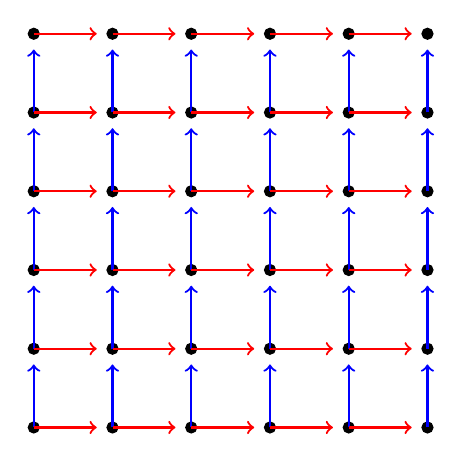
\begin{tikzpicture}
      \foreach \x in{0,...,5} { 
        \foreach \y in{0,...,5} {
          \filldraw (\x, \y) circle (2pt);
        }
      }

      \foreach \x in {0,...,5} {
        \foreach \y in {0,..., 4} {
          \draw[->, blue, thick] (\x, \y) -- (\x, \y+.8);
        }
      }
      \foreach \x in {0,...,4} {
        \foreach \y in {0,..., 5} {
          \draw[->, red, thick] (\x, \y) -- (\x+.8, \y);
        }
      }
    \end{tikzpicture}
  \end{center}
\item Dla grupy cyklicznej rzędu $p$ z generatorem $\color{red}s$ graf Cayleya to $p$-kąt
  \begin{center}
    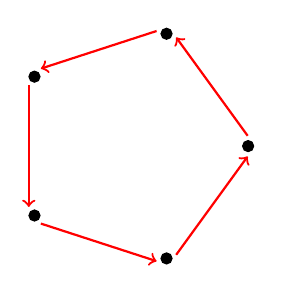
\begin{tikzpicture}
      \foreach \i in {0,..., 4} {
        \filldraw ( 360 /5 * \i :1.5) circle (2pt);
        \draw[->, red, thick] (360/5*\i + 5:1.5) -- (360/5*\i + 360/5 - 5:1.5);
      }
    \end{tikzpicture}
  \end{center}
\item {\color{red}\Large TO DO} parkietarz kwadratami
\end{example}

Każdy graf Cayleya jest \buff{spójny}, bo jego krawędzie to mnożenie przez generatory. Dodatkowo, grupa $G$ działa na nim przez \hl{automorfizmy zachowując krawędzie oraz ich etykiety}. To znaczy, że krawędż z wierzchołkami \begin{tikzcd}g\arrow[r, "s"]&gs\end{tikzcd} pod działaniem elementu $\gamma \in G$ staje się \begin{tikzcd}\gamma g\arrow[r, "s"] & \gamma gs\end{tikzcd}.

Jeśli każdą krawędź w grafie Cayleya potraktujemy jako odcinek długości $1$, to możemy na nim zdefiniować metrykę która jako odległość dwóch punktów przyjmuje długość najkrótszej ścieżki między nimi. Ta metryka na wierzchołkach pokrywa się z \buff{metryką słów} na grupie $G$ o generatorach $S$, której graf rozpatrujemy. Przy takiej metryce działanie grupy $G$ jest więc działaniem nie tylko przez automorfizmy, ale przez izometrie (lewa-niezmienniczość).


\section{25.02.2025}{Produkty i koprodukty kategorii}

\subsection{O obiektach początkowych i końcowych słów kilka}

\begin{definition}{obiekt początkowy i końcowy}{}
  Powiemy, że obiekt $C\in \Cc_0$ jest \buff{początkowy}, jeśli dla każdego $D\in\Cc_0$ istnieje dokładnie jeden morfizm $C\to D$, $|\Cc(C, D)|=1$. Analogicznie definiujemy \buff{obiekt końcowy} $C$: $\forall\;D\in\Cc_0\;|\Cc(D, C)|=1$.
\end{definition}

\begin{example}[m]
  \item W kategorii, której obiektami jest odcinek $\Cc_0=[0,1]$, a morfizmy to relacja $\leq$ obiektem początkowym jest $0$, a końcowym - $1$.
  \item W kategorii zbiorów obiektem początkowym jest $\emptyset$, a obiektem końcowym jest singleton.
  \item W $Gr$ grupa trywialna jest zarówno obiektem początkowym jak i końcowym.
  \item Kategoria, która ma dwa obiekty bez morfizmów między nimi nie ma obiektu końcowego ani początkowego.
\end{example}

\begin{fact}{}{}
  Obiekty końcowe i początkowe, jeśli istnieją, to są jedyne z dokładnością do izomorfizmu.
\end{fact}

\begin{proof}
  Niech $C$ i $C'$ będą obiektami końcowymi kategorii $\Cc$. Wiemy, że $\Cc(C, C)=\{id_C\}$, czyli komutujący diagram
  \begin{center}
    \begin{tikzcd}
      C \arrow[rr, "id_C"]\arrow[dr, "\exists!f" below left] & & C\\ 
                           & C'\arrow[ur, "\exists!g" below right]
    \end{tikzcd}
  \end{center}
  daje $g\circ f=id_C$. Analogiczny diagram daje $f\circ g=id_{C'}$. Stąd $f$ i $g$ to para wzajemnie odwrotnych izomorfizmów między $C$ i $C'$
\end{proof}

\subsection{(Ko)granice funktorów a (ko)produtky}

Niech $F:\mathcal{I}\to \Cc$ będzie funktorem, gdzie o kategorii $\mathcal{I}$ myślimy jako o kategorii indeksów. Przez $\Cc^{\mathcal{I}}$ oznaczmy kategorię wszystkich takich funktorów. 
Powiemy, że funktor $C$ jest stały, jeżeli $C(i)=C$ dla każdego $i\in\mathcal{I}_0$ oraz $C(f)=id_C$ dla każdego morfizmu.

Budujemy kategorię, której 
\begin{itemize}
  \item obiekty to wszystkie naturalne przekształcenia funktora $F$ w funktory stałe $C$, $\phi:F\implies C$, czyli komutujące diagramy (kostożki) 
    \begin{center}
      \begin{tikzcd}
        F(i)\arrow[rr, "F(f)"]\arrow[dr, "\phi_i" below left] & & F(j)\arrow[dl, "\phi_j"]\\ 
                                                  & C
      \end{tikzcd}
    \end{center}
  \item a morfizmy to strzałki $C\to D$ takie, że diagram
    \begin{center}
      \begin{tikzcd}
        C\arrow[rr] & & D\\ 
                    & F\arrow[ur, Rightarrow, blue, "\phi" below right]\arrow[ul, Rightarrow, orange, "\psi" below left]
      \end{tikzcd}
    \end{center}
    komutuje.
\end{itemize}

Diagram wyżej można rozpisać jako:
\begin{center}
  \begin{tikzcd}[column sep=large]
    & F(i)\arrow[d] \arrow[ddl, "\phi_i" above left, blue]\arrow[ddr, "\psi_i" above right, orange] \\ 
    & F(j)\arrow[dl, "\phi_j" above, blue]\arrow[dr, "\psi_j" above, orange]\\ 
    D & & C\arrow[ll]
  \end{tikzcd}
\end{center}

\begin{definition}{kogranica funktora}{}
  \buff{Kogranicą} (\acc{granica prosta}) funktora $F$, $\varinjlim F$, nazywamy obiekt początkowy w wyżej zdefiniowanej kategorii naturalnych przekształceń. 
  % \buff{Granica} (\acc{granica odwrotna}) to wtedy obiekt końcowy powyższej kategorii ze wszystkimi strzałkami zdualizowanymi $\varprojlim F$.
\end{definition}

Diagram wyżej możemy zdualizować i zamiast rozpatrywać naturalne przekształcenia $\phi:F\implies C$ możemy rozważyć naturalne przekształcenia $\phi:C\implies F$, czyli diagramy (stożki)
\begin{center}
  \begin{tikzcd}
    & C \arrow[dl, "\phi_i" above left] \arrow[dr, "\phi_j" above right]\\ 
    F(i)\arrow[rr, "F(f)" below] & & F(j)
  \end{tikzcd}
\end{center}
z morfizmami {definiowanymi analogicznie. 

\begin{definition}{granica funktora}{}
  \buff{Granica} (\acc{granica odwrotna}) to obiekt końcowy powyższej kategorii stożków, $\varprojlim F$.
\end{definition}

% {\color{red}tutaj jest zdjecie
%
% przyklad dla kategorii zbiorów
%
% ja chyba chce wziąć dwuelementową kategorię $\mathcal{I}$ i tutaj policzyć, jeśli $F(1)=G$, a $F(2)=H$.
% }
%
Rozważmy kategorię $\mathcal{I}$, która ma dwa obiekty $\mathcal{I}_0=\{0,1\}$. Niech $F:\mathcal{I}\to Set$ będzie funktorem, dla którego $F(0)=A$, a $F(1)=B$. Niech $\phi$ oraz $\psi$ będzie parą naturalnych przekształceń, dla których
\begin{center}
  \begin{tikzcd}[column sep=large, row sep=large]
     & \varinjlim F\arrow[dl, "\phi_0" above left] \arrow[dr, "\phi_1"] \\ 
    F(0)=A & D \arrow[l, "\psi_0"] \arrow[r, "\psi_1" below right] \arrow[u, "\exists!f", dashed] & F(1)=B
  \end{tikzcd}
\end{center}
gdzie pionowa strzałka istnieje i jest jedyna, bo $\varinjlim F$ to obiekt końcowy. Jeśli weźmiemy $\varinjlim F=A\times B$, a $\phi_0=\pi_A$ oraz $\phi_1=\pi_B$ będą rzutami i $f(d)=(\psi_0(d), \phi_1(d))$, to diagram nadal jest prawdziwy. 

Granica odwrotna tego samego funktora, to z kolei suma rozłączna $A\sqcup B$, bo diagram
\begin{center}
  \begin{tikzcd}[column sep=large, row sep=large]
    F(0)=A\arrow[r, "\psi_0"]\arrow[dr, "\phi_0=i_A" below left] & D & F(1)=B\arrow[l, "\psi_1" above]\arrow[dl, "\phi_1=i_B"]\\ 
                                                       & \varprojlim F= A\sqcup B \arrow[u, dashed, "\exists!f"]
  \end{tikzcd}
\end{center}
gdzie $f(x)=\phi_0(x),$ jeśli $x\in A$ oraz $f(x)=\psi_1(x)$ jeśli $x\in B$, komutuje.

\begin{definition}{(ko)produkt}{}
  \buff{Produktem} obiektów $A$ i $B$ kategorii $\Cc$ nazywamy granicę prostą (kogranicę) funktora $F:\mathcal{I}\to \Cc$ dla $\mathcal{I}$ oraz $F$ jak wyżej.

  \buff{Koproduktem} obiektów $A$ i $B$ kategorii $\Cc$ nazywamy granicę odwrotną (granicę) funktora $F:\mathcal{I}\to\Cc$
\end{definition}

\begin{example}[m]
  \item W kategorii grup produkt to iloczyn kartezjański dwóch grup, tak jak w kategorii zbiorów, tj. dla grup $A,G,H$ komutuje diagram
    \begin{center}
      \begin{tikzcd}[column sep=large, row sep=large]
        & G\times H\arrow[dl, "\pi_G" above left]\arrow[dr, "\pi_H"]\\ 
        G & A\arrow[l, "g"]\arrow[r, "h"]\arrow[u, "g\times h" below] & H
      \end{tikzcd}
    \end{center}
    Koprodukt to z kolei produkt wolny tych dwóch grup:
\begin{center}
  \begin{tikzcd}[column sep=large, row sep=large]
    G\arrow[r, "g"]\arrow[dr, "i_G" below left] & A & H\arrow[l, "h" above]\arrow[dl, "i_H"]\\ 
                                                       & H\ast G \arrow[u, dashed, "\exists!f"]
  \end{tikzcd}
\end{center}
gdzie $f$ nakłada na litery słów $G\ast H$ pochodzące z $G$ morfizm $g$, a na litery pochodzące z $H$ - morfizm $h$.
  \item Niech $F:\mathcal{I}\to (P, \leq)$ z dwuobiektowej kategorii $\mathcal{I}$ w zbiór uporządkowany. Wtedy jeśli mamy diagram 
    \begin{center}
      \begin{tikzcd}
         & \varinjlim F\arrow[dr]\arrow[dl] \\ 
        F(0)=a & d \arrow[l]\arrow[r]\arrow[dashed, u] & F(1)=b
      \end{tikzcd}
    \end{center}
    to znaczy, że $d\leq a$, $d\leq b$ oraz $d\leq \varinjlim{F}$. Żeby więc miało to sens dla dowolnego $d\leq a,b$ to $\varinjlim F=\inf\{a,b\}$. Analogicznie dostajemy, że $\varprojlim F=\sup\{a,b\}$.

  \item Jeśli $\mathcal{I}$ jest kategorią o nieskończenie wielu obiektach bez morfizmów między różnymi obiektami, a $F:\mathcal{I}\to Set$ jest funktorem w kategorię zbiorów, to wówczas kogranicą tego funktora jest nieskończony iloczyn kartezjański $\prod_{i\in\mathcal{I}_0}F(i)$, a granicą - nieskończona suma rozłączna $\bigsqcup_{i\in\mathcal{I}_0}F(i)$.
\end{example}

% kategoria nieskończenie wiele elementów, ale bez strzałek (jako $\mathcal{I}$)
 % Niech $C$ oraz $C'$ będą kogranicami tego samego funktora. Z definicji mamy
% \begin{center}
%   \begin{tikzcd}[column sep=large, row sep=large]
%     & F(i)\arrow[dr, "\phi_i"]\arrow[d, "\psi_i"]\arrow[dl, "\phi_i" above left] \\ 
%     C & C'\arrow[l, "\exists g" above] & C\arrow[ll, bend left=20, "id"] \arrow[l, "\exists f" above]
%   \end{tikzcd}
% \end{center}

\begin{fact}{}{}
  Granica i kogranica funktora, jeśli istnieje, to jest jedyna z dokładnością do izomorfizmu. Stąd również produkty i koprodukty są unikalne.
\end{fact}

\begin{proof}
  Wynika z uniwersalności obiektów końcowych i początkowych.
\end{proof}

% tutaj liczby p-adyczne
% ekwalizator, koekwalizator
%
% \begin{definition}{surjekcja, epimorfizm}{}
%   Jeśli kategoria ma obiekt początkowy równy obiektowi końcowemu...
% \end{definition}

\begin{example}
  Rozważmy funktor $F:\mathcal{I}^{op}\to Grp$, gdzie $\mathcal{I}=(\N, \leq)$ taki, że dla każdych $i,j\in\N$, $i\leq j$ mamy
  \begin{center}
    \begin{tikzcd}[column sep=large]
      F(j)=\Z/p^j\Z\arrow[r, "F(i\to j)=q"] & F(i)=\Z/p^i\Z
    \end{tikzcd}
  \end{center}
  gdzie $q$ to morfizm ilorazowy.

  Liczby $p$-adyczne to rozszerzenie liczb wymiernych różne od liczb rzeczywistych i zespolonych. Całkowite liczby $p$-adyczne to szeregi
  $$\sum_{i=k}^\infty a_ip^i,$$
  gdzie $k\in\N$ oraz $0\leq a_i < p$. Okazuje się, że całkowite liczby $p$-adyczne, $\Z_p$, można zdefiniować jako granicę funktora $F$:
  \begin{center}
    \begin{tikzcd}
      & & \Z_p \arrow[dll]\arrow[dl]\arrow[d]\arrow[drr]\arrow[drrr] \\ 
      ...\arrow[r] & \Z/p^n\Z\arrow[r] & \Z/p^{n-1}\Z\arrow[r] & ... \arrow[r]& \Z/p^2\arrow[r] & \Z/p\Z
    \end{tikzcd}
  \end{center}
  Granica prosta takiego funktora jest trywialna, ale możemy rozważyć inny funktor,z kategorii $\Z$ z porządkiem, tzn: $G:\Z\to Grp$ taki, że $G(n)=\Z/p^n\Z$, natomiast strzałkę $n+1\to n$ przekształcamy na odwzorowanie
  $$\Z/p^n\Z\ni x\mapsto p\cdot x\in \Z/p^{n+1}\Z.$$
  Wtedy granicą prostą $G$ jest $C_{p^\infty}$ - pierwiastki $p^n$-tego stopnia z $1$, dla dowolnego $n$. 
\end{example}

\subsection{Obiekty i kategorie monoidalne}

\buff{Monoid} $(M, \star, 1)$ to struktura algebraiczna z binarną operacją oraz elementem neutralnym. Dodatkowo, komutować ma diagram 
\begin{center}
  \begin{tikzcd}
    M^3\arrow[r, "\star\times id"]\arrow[d, "id\times\star" left] & M^2\arrow[d, "\star"]\\ 
    M^2\arrow[r, "\star"] & M
  \end{tikzcd}
\end{center}
co znaczy, że działanie jest łączne.

\begin{definition}{obiekt monoidalny, kategoria monoidalna}{}
  Niech $\Cc$ będzie kategorią z produktem i elementem początkowym. Niech $M\in \Cc$ będzie obiektem, dla którego mamy $\mu:M^2\to M$ oraz $\epsilon: \{1\}\to M$ takie, że komutują diagramy
  \begin{center}
    \begin{tikzcd}[row sep=large, column sep=large]
      M^3\arrow[r, "\mu\times id"]\arrow[d, "id\times \mu" left] & M^2\arrow[d, "\mu"]\\ 
      M^2\arrow[r, "\mu" below] & M
    \end{tikzcd}
  \end{center}
  \begin{center}
    \begin{tikzcd}[row sep=large, column sep=large]
      M\arrow[r, "\epsilon\times id"]\arrow[d, "id\times \epsilon" left]\arrow[dr, "=" above right] & M^2\arrow[d, "\mu"]\\ 
      M^2\arrow[r, "\mu" below] & M
    \end{tikzcd}
  \end{center}
  Wtedy $M$ jest \buff{obiektem monoidalnym}.
  
  Obiekt monoidalny w kategorii $Cat$ nazywa się \buff{kategorią monoidalną}.
\end{definition}

\begin{example}[m]
\item Dowolna kategoria $\Cc$ z koproduktem i obiektem końcowym jest kategorią monoidalna.
\item Kategoria endofunktorów ma strukturę monoidalną. To znaczy, jeśli mamy dwa endofunktory $F, G\in End(\Cc)$, to potrafimy je złożyć w dobry sposób.

  Funktor $T\in End(\Cc)$ oraz dwa naturalne przekształcenia $\mu:T^2\to T$, $\epsilon: Id\to T$, nazywa się \buff{monadą}.
\end{example}

% Czy $S^n\vee S^n$ to produkt czy produkt w kategorii $Toph_\star$. tutaj jakies zdjecie








\chapter{Niezmienniki izometrii}

\section{16.10.2024}{Końce (w nieskończoności) grup przestrzeni}

Zanim zaczniemy, zróbmy szybką motywację, czyli graf Cayleya grupy $\Z$ z jednym generatorem (rysunek \ref{Z graf})
\begin{figure}[H]\center
  
\begin{tikzpicture}
    \draw[dashed] (-.75, 0)--(0,0);
    \draw[dashed] (5,0)--(5.75, 0);
    \draw (0, 0)--(5, 0);
    \foreach \i in {0, 1, ..., 5} \fill (\i, 0) circle (2pt);
  \end{tikzpicture}

  \caption{\label{Z graf}Graf Cayleya grupy $\Z$ ma dwa końce.}
\end{figure}
który ma "dwa końce". Natomiast grupa wolna $F_2$ o dwóch generatorach ma "nieskończenie wiele końców" (rysunek \ref{graf F2}).
\begin{figure}[H]\center
  \begin{tikzpicture}
    \tikzmath {
      function drawLine (\x, \y, \scale, \step) {
        \step = \step -1;
        if \step >= 0 then {
          {
            \draw (\x, \y-0.8*\scale)--(\x, \y+0.8*\scale);
            \draw (\x-0.8*\scale, \y)--(\x+0.8*\scale, \y);
          };
          \scale = \scale *0.45;
          drawLine(\x - \scale, \y, \scale, \step);
          drawLine(\x + \scale, \y, \scale, \step);
          drawLine(\x, \y - \scale, \scale, \step);
          drawLine(\x, \y + \scale, \scale, \step);
        };
      };
      drawLine(0, 0, 4, 4);
    }
  \end{tikzpicture}
  \caption{\label{graf F2}Graf Cayleya grupy wolnej $F_2$ ma nieskończenie wiele końców.}
\end{figure}
Z drugiej strony, grupa $\Z^2$ ma jeden koniec: jeśli weźmiemy dwa bardzo odległe od siebie obszary, to one są ze sobą połączone, chociaż jest to połączenie "bardzo odległe" (obrazek \ref{graf Z2}).
\begin{figure}[H]\center
  \begin{tikzpicture}
    \tikzmath{
      for \x in {-3, ..., 3} {
        {
          \draw (\x, 3)--(\x, -3);
          \draw[dashed] (\x, 3)--(\x, 3.5);
          \draw[dashed] (\x, -3)--(\x, -3.5);
          \draw (-3, \x)--(3, \x);
          \draw[dashed] (-3.5, \x)--(-3, \x);
          \draw[dashed] (3, \x)--(3.5, \x);
        };
        for \y in {-3, ..., 3} {
          {\fill (\x, \y) circle (2pt);};
        };
      };
    }
    
    \draw[blue, thick, dashed] (-4, 0) to[out=-90, in=170]
      (-3.5, -4) to[out=-10, in=190] 
      (3.5, -4) to[out=10, in=-90]
      (4, 0);
    \draw[blue, thick, dashed] (-6, 0) to[out=-90, in=170]
      (-5.5, -5) to[out=-10, in=190]
      (5.5, -5) to[out=10, in=-90]
      (6, 0);

    \draw[orange, dashed, thick] (5, 0) ellipse (1 and 1.8);
    \draw[orange, dashed, thick] (-5, 0) ellipse (1 and 1.8);

    \node at (-6, 3) {\begin{varwidth}{3.3cm}\begin{center}\color{orange}dwa bardzo odległe obszary\end{center}\end{varwidth}};

    \draw[orange, ->, thick] (-7, 2.2) to[out=-90, in=180] (-6.2, 0);
    \draw[orange, ->, thick] (-4.3, 3.4) to[out=30, in=90] (5, 2);

    % \node[blue] at (0, -4.9) {połączone, choć nie bezpośrednio};
    \draw[decoration={text along path, text={połączone, choć nie bezpośrednio}, text align=center, text color=blue}, decorate] 
      (-3.5, -4.8) to[out=-10, in=190] (3.5, -4.8); 
  \end{tikzpicture}
  \caption{\label{graf Z2}Graf Cayleya grupy $\Z^2$ ma jeden koniec.}
\end{figure}
Każda przestrzeń skończona, np. graf Cayleya grupy skończonej, ma $0$ końców.

Chcemy z liczby końców przestrzeni (albo przestrzeni końców) uczynić tzw. niezmiennik asymptotyczny, czyli cechę niezmienną na quazi-izometrie właściwych geodezyjnych przestrzeni metrycznych, a co za tym idzie - przestrzeni skończenie generowanych.

\subsection{Granica odwrotna}

\begin{definition}{zbiór skierowany}{}
  Zbór z częściowym porządkiem $(\Lambda, \leq)$ jest \buff{skierowany}, gdy dla dowolnych $\lambda_1,\lambda_2\in\Lambda$ istnieje $\lambda\in\Lambda$ takie, że $\lambda\geq \lambda_1$ oraz $\lambda\geq \lambda_2$.
\end{definition}

% {\large\color{red}ciągi odwrotne}

\begin{definition}{system odwrotny}{}
  \buff{System odwrotny} nad zbiorem skierowanym $\Lambda$ to rodzina zbiorów 
  $$\mathfrak{X}:=\{X_\lambda\;:\;\lambda\in\Lambda \}$$
  oraz rodzina odwzorowań
  $$\mathcal{F}:=\{f_{\lambda\mu}:X_\mu\to X_\lambda\;:\;\lambda\leq\mu \}$$
  takich, że 
  \begin{enumerate}
    \item dla dowolnego $\lambda$ mamy funkcję identycznościową: $f_{\lambda\lambda}=id_{X_\lambda}$
    \item dla dowolnych $\lambda\leq\mu\leq\nu$ złożenia zachowują się dobrze: $f_{\lambda\nu}=f_{\lambda\mu}\circ f_{\mu\nu}$.
  \end{enumerate}
\end{definition}

Będziemy oznaczać: $\boldsymbol{\underline{X}:=(\Lambda, \mathfrak{X}, \mathcal{F})}$

\begin{definition}{granica odwrotna}{granica odwrotna}
  Granicą odwrotną systemu $\underline{X}$ nazywamy zbiór
  $$\varprojlim\underline{X}=\varprojlim(\Lambda, \mathfrak{X}, \mathcal{F}):=\{\xi\in\prod_{\lambda\in\Lambda}X_\lambda\;:\;(\forall\;\lambda'\leq\lambda)\;\xi_{\lambda'}=f_{\lambda'\lambda}(\xi_\lambda)\}.$$
  Elementy $\xi$ jak wyżej nazywamy \hl{niciami} (threads) w $\underline{X}$.
\end{definition}

% \begin{definition}{odwzorowania graniczne}{}
Odwzorowania 
$$f_\lambda:\varprojlim\underline{X}\to X_\lambda$$ 
takie, że $f_\lambda(\xi)=\xi_\lambda$ nazywamy \buff{odwzorowaniami granicznymi}.
O odwzorowaniach granicznych można myśleć jako o odwzorowaniach, które pytają "kim byłem w czasie $\lambda$".

\begin{center}
  \begin{tikzcd}
    X_1 & X_2 \arrow[l] & X_3\arrow[l] & X_4 \arrow[l] & ... \arrow[l]\\ 
        & & \varprojlim\underline{X}\arrow[ull]\arrow[ul]\arrow[u]\arrow[ur]\arrow[urr]
  \end{tikzcd}
\end{center}

Dla $\lambda\leq\mu$ diagram 
\begin{center}
  \begin{tikzcd}
    &\underset{\leftarrow}{\lim}\underline{X}\arrow[dl, "f_\lambda" above left]\arrow[dr, "f_\mu"]\\ 
    X_\lambda && X_\mu\arrow[ll, "f_{\lambda\mu}"]
  \end{tikzcd}
\end{center}
zawsze komutuje.

% \subsection{Toopologia granicy odwrotnej}

Kiedy zbiory $X_\lambda$ są przestrzeniami topologicznymi, zaś $f_{\lambda\mu}$ są ciągłe, to na granicy odwrotnej $\varprojlim\underline{X}$ rozważamy również topologię graniczną. Jest to topologia dziedziczona z topologii produktowej na $\prod_{\lambda\in\Lambda}X_\lambda$. 

\hl{Bazą tej topologii są zbiory postaci }\hl{$f_\lambda^{-1}(U)$ dla $\lambda\in\Lambda$ i otwartych $U\subseteq X$.}

\begin{fact}{}{}
  Granica odwrotna $\varprojlim\underline{X}$ jest:
  \begin{enumerate}
    \item domkniętym podzbiorem $\prod_{\lambda\in\Lambda}X_\lambda$, jeśli $X_\lambda$ są Hausdorffa,
      % gdy przestrzenie $X_\lambda$ są Hausdorffa, to $\varprojlim \underline{X}$ jest domkniętym podzbiorem w $\prod_{\lambda\in\Lambda}X_\lambda$.
    \item zwarta i metryczna, jeśli $X_\lambda$ takie są,
    \item zwarta i metryczna, jeśli $\Lambda$ jest przeliczalny, a $X_\lambda$ są skończone (z topologią dyskretną).
  \end{enumerate}
\end{fact}

W ostatnim przypadku $\varprojlim \underline{X}$ nie jest przestrzenią dyskretną, pomimo, że wszystkie zbiory po których bierzemy granicę takie były. Rozważmy następujący przykład, w którym $\Lambda=\N$, a wszystkie $X_\lambda$ są skończone dyskretne, natomiast $\varprojlim \underline{X}$ jest niedyskretne i nieskończone.

% Gdy przestrzenie $X_\lambda$ są zwarte i metryczne, to wówczas $\varprojlim\underline{X}$ też jest zwarta i metryczna. W szczególności, gdy $X_\lambda$ są skończone (z topologią dyskretną), zaś $\Lambda$ jest przeliczalny, to wówczas $\varprojlim\underline{X}$ jest \hl{przestrzenią zwartą i metryczną}. Na ogół nie jest też przestrzenią dyskretną, mimo że wszystkie zbiory po których bierzemy granicę takie były (bazą topologii są przeciwobrazy punktów $\{\xi\in\varprojlim\underline{X}\;:\;\xi_\lambda=x\}=f^{-1}_\lambda(x)$).

\begin{example}{}{}
  Niech $\Lambda=(\N, \leq)$ i niech $X_k$ będzie zbiorem wszystkich ciągów $0-1$ długości $k$. Dla $k\leq m$ rozważamy 
  $$f_{km}:X_m\to X_k$$
  będące obcięciem ciągu długości $m$ do początkowego ciągu długości $k$. Dostajemy wówczas system odwrotny $\underline{X}=(\N, \{X_k\}, \{f_{km}\})$ zbiorów skończonych. Wówczas $\varprojlim\underline{X}$ jest homeomorficzny ze zbiorem Cantora.
\end{example}

\subsection{Przestrzeń końców}

Na tym wykładzie będziemy zajmować się $X$, które są właściwymi geodezyjnymi przestrzeniami metrycznymi. Takimi przestrzeniami są np. grafy Cayleya grup skończenie generowalnych. Przez zbiór $\mathcal{K}$ będziemy rozumieć rodzinę wszystkich zwartych podzbiorów $K\subseteq X$ z porządkiem inkluzji.

% Będziemy zajmować się $X$ które są przestrzeniami metrycznymi, geodezyjnymi właściwymi, np. grafami Cayleya grup skończenie generowanych. $\mathcal{K}$ to będzie rodzina wszystkich zwartych podzbiorów $K\subseteq X$ z porządkiem inkluzji.

\begin{definition}{podzbiór współkońcowy}{}
  Podzbiór $M\subseteq\Lambda$ zbioru skierowanego $\Lambda$ nazywamy \buff{współkońcowym}, jeśli 
  $$(\forall\;\lambda\in\Lambda)(\exists\;\mu\in M)\;\lambda\leq\mu,$$ 
  wtedy $(M, \leq)$ też jest zbiorem skierowanym. Dla $\underline{X}=(\Lambda, \mathfrak{X}, \mathcal{F})$ niech 
  $$\underline{X}_{|M}=(M, \{X_\lambda\;:\;\lambda\in M\}, \{f_{\mu\mu'}\in\mathcal{F}\;:\;\mu,\mu'\in M\})$$
  będzie obcięciem $\underline{X}$ do $M$. Wtedy $\underline{X}_{|M}$ jest systemem odwrotnym nad $M$.
\end{definition}

\begin{fact}{}{}
  $$\varprojlim\underline{X}=\varprojlim\underline{X}_{|M}$$
  Przez bijekcją polegającą na obcinaniu nici do $M$. Jest ona jednocześnie homomorfizmem.
\end{fact}

\begin{conclusion}{}{} 
  Jeśli $X_\lambda$ są zwarte i metryczne, zaś $\Lambda$ posiada przeliczalny podzbiór współkońcowy, to $\varprojlim\underline{X}$ jest zwarta i metryczna.
\end{conclusion}

\begin{example}
Rodzina zbiorów zwartych $\mathcal{K}$ posiada współkońcowy podciąg $K_i:=B_{i\cdot R}(x_0)$ dla $R>0$ i pewnego $x_0\in X$.
  \end{example}
    
Dla dowolnego $K\in\mathcal{K}$ niech \hl{$\Pi_K^X$ będzie zbiorem nieograniczonych komponent spójności w dopełnieniu $X-K$}.

Przestrzeń geodezyjna jest lokalnie drogowo spójna i każda jej otwarta podprzestrzeń również jest lokalnie drogowo spójna. Stąd każde $X-K$ też jest lokalnie drogowo spójna. W lokalnie drogowo spójnych przestrzeniach komponenty spójności to to samo co komponenty drogowej spójności.\medskip

Dla $K\subseteq K'$, każda nieograniczona komponenta spójności $C'\subseteq X-K'$ zawiera się w dokładnie jednej nieograniczonej komponencie spójności $C\subseteq X-K$. Dostajemy więc odwzorowanie 
$$f_{KK'}:\Pi_{K'}^X\to \Pi_K^X$$
takie, że $f_{KK'}(C')=C$. 

Trójka $(\mathcal{K}, \{\Pi_K^X\;:\;K\in\mathcal{K}\},\{f_{KK'}\;:\;K'\subseteq K\})$ tworzy system odwrotny nad zbiorem skierowanym $\mathcal{K}$:
\begin{center}
  \begin{tikzcd}
    \Pi_K^X & \Pi_{K'}^X\arrow[l, "f_{KK'}"] & \Pi_{K''}^X\arrow[l, "f_{K'K''}"]
  \end{tikzcd}
\end{center}

\begin{fact}{}{}
  Dla każdego $K\in\mathcal{K}$ zbiór $\Pi_K^X$ jest skończony.
\end{fact}

\begin{proof}
  Weźmy dowolny $K\in\mathcal{K}$ i $x_0$ oraz $r$ takie, że 
  $$K\subseteq B_r(x_0).$$ 
  Niech $R>r$ i rozważmy zwartą kulę $B_R(x_0)$. Każda nieograniczona komponenta $C$ spójności w $X-K$ przecina niepusto sferę $S_R(x_0)$, bo $X$ jest geodezyjna, a więc lokalnie drogowo spójna...

  Zatem przekrój $C\cap B_R(x_0)$ jest niepusty. Wtedy rodzina 
  $$\{C\cap B_R(x_0)\;:\;C\text{ dowolna komponenta dopełnienia }X-K\}\cup \{\overline{B_R}(x_0)=B_R(x_0)-S_R(x_0)\}$$
  pokrywa $B_R(x_0)$. Dodatkowo, jest to otwarte pokrycie, bo komponenty spójności lokalnie spójnej przestrzeni są otwartymi podzbiorami w tej przestrzeni. 

  Ze zwartości $X$ to pokrycie posiada skończone podpokrycie, ale z drugiej strony każdy zbiór postaci $C\cap B_R(x_0)$ dla nieograniczonych komponent musi przetrwać w każdym podpokryciu, bo zawiera punkty które należą tylko do niego. Stąd nieograniczonych komponent jest skończenie wiele.
\end{proof}

\begin{definition}{przestrzeń końców}{}
  Zbiorem (przestrzenią) końców, $Ends(X)$, właściwej geodezyjnej przestrzeni metrycznej $X$ nazywamy granicę odwrotną
  $$\Ends(X)=\varprojlim(\Pi^X)=\varprojlim(\mathcal{X}, \{\Pi_K^X\}, \{f_{KK'}\}),$$
  gdzie $\Pi_K^X$ to nieograniczone komponenty w $X-K$.  Jest to zwarta przestrzeń metryczna.
\end{definition}

\begin{example}[m]
  \item $\Ends(\text{ograniczone}))=\emptyset$
  \item $\Ends(\Z^2)=\{\star\}$ to punkt w nieskończoności kraty
  \item $\Ends(\Z)=\{-\infty, \infty\}$ i jest równoliczny z $\Ends(\R)$
  \item zbiór końców drzewa $k$-regularnego, dla $k\geq 3$, jest izomorficzny ze zbiorem Cantora
  \item dla nieskończonych grup skończenie generowanych $G_1$, $G_2$ przestrzeń końców $\Ends(G_1\star G_2)$ jest nieskończonym zbiorem
\end{example}




\section{23.10.2024}{Przestrzeń końców jest niezmiennikiem q.i.}

Celem dzisiejszego wykładu będzie udowodnienie poniższego twierdzenia.

\begin{theorem}{}{niezmienniczoscEnds} 
  Przestrzeń końców $Ends(X)$, a w szczególności ich liczba, jest niezmiennikiem quasi-izometrii geodezyjnych przestrzeni właściwych (przestrzenie końców są wtedy homeomorficzne). %Takie q.i. przestrzenie mają homeomorficzne przestrzenie końców.
\end{theorem}

\subsection{Alternatywny opis przestrzeni końców (promienie)}

Przypomnijmy, że jeśli $X$ jest właściwa przestrzenią geodezyjną, to jest również lokalnie drogowo spójna. Czyli otwarte podzbiory $U\subseteq X$ są spójne $\iff$ są drogowo spójne.

\begin{definition}{promień, współkońcowość promieni}{}
  \buff{Właściwy promień} (eng. proper ray) w $X$ to dowolne ciągłe odwzorowanie $\rho:[0,\infty)\to X$ takie, że 
  $$\lim_{t\to\infty}d_X(\rho(0), \rho(t)),$$
  odległość mierzona od początku $\rho$ ucieka do nieskończoności wraz z oddalaniem się od $0$.

  \hl{Zbiór wszystkich promieni w $X$ oznaczamy $\rho^X$.}

  Powiemy, że dwa promienie $\rho_1,\rho_2$ są współkońcowe ($\rho_1\wspolkon\rho_2$), jeśli dla dowolnego zwartego $K\subseteq X$ istnieje $R>0$ taki, że $\rho_1([R, \infty))$ oraz $\rho_2([R, \infty))$ leżą w tej samej komponencie $X-K$.
\end{definition}

Relacja współkońcowości promieni na zbiorze $\rho^X$ jest relacją równoważności.

\begin{fact}{}{}
  Zbiór klas abstrakcji $\rho^X/\wspolkon$ w naturalny sposób utożsamia się z $Ends(X)$.
\end{fact}

\begin{proof}
  Weźmy $\rho\in\rho^X$ takie, że dla każdego $K\subseteq X$ mamy jedyną komponentę $C_K^\rho\in\Pi_K^X$ w dopełnieniu zbioru $K$ w $X$ do której należy $\rho([R,\infty))$ dla dostatecznie dużych $R$. Wtedy ciąg 
  $$(C_K^\rho)_{K\in\mathcal{K}}$$ 
  jest nicią [\ref{def:granica odwrotna}] w systemie odwrotnym $(\mathcal{K},\Pi^X,)f_{KK'})$ . 

  Współkońcowe promienie wyznaczają tę samą nić, więc istnieje dobrze określone odwzorowanie 
  $$\beta:\rho^X/\wspolkon \to \Ends(X)$$
  $$\beta([\rho]_{\wspolkon})=(C_K^{\rho})_{K\in\mathcal{K}}\in \Ends(X)$$
  $\beta$ jest różnowartościowe, bo dla niewspółkońcowych $\rho_1,\rho_2$ istnieje $K\subseteq X$ takie, że $C_K^{\rho_1}\neq C_K^{\rho_2}$, a wtedy nici $\beta([\rho_1])\neq \beta([\rho_2])$.

  Wystarczy przekonać się, że $\beta$ jest surjekcją. 

  Niech $\xi=(\xi_K)\in\Ends(X)$ będzie dowolną nicią. Szukamy promienia który na nie przechodzi. Dla każdego $n\in\N$ wybieramy punkt $y_n\in \xi_{B_n}$, gdzie $\xi_{B_n}$ to nieograniczona komponenta w $X-B_n$ dla $B_n=B_n(x_0)$ przy ustalonym $x_0$. 

  Określmy $\rho=[y_0,y_1]\cup[y_1,y_2]\cup...$ mając na myśli odwzorowanie $\rho$ które odcinek $[n, n+1]$ przeprowadza na geodezyjną od $y_n$ do $y_{n+1}$. Dla takiego $\rho$ mamy $C_{B_n}^\rho=\xi_{B_n}$. Dla dowolnego innego $K\in \mathcal{K}$ z racji, że istnieje kula taka, że $K\subseteq B_n$ to dla pewnego $n$ zarówno $C_K^\rho$ jak i $\xi_K$ to ta sama komponenta w $X_K$, zawierająca $\xi_{B_n}$.
\end{proof}

Na $\rho^X/\wspolkon$ mamy topologie indukowana przez bijekcję $\beta$ z topologii $\Ends(X)$. Baza tej topologii są zbiory postaci 
$$\{U_C^K\;:\;K\in\mathcal{K}\text{ i }C\in\Pi_K^X\},$$ 
$U_C^K=\{[\rho]\;:\;\rho([R, \infty))\subset C\}$ dla pewnego $R$.


Wróćmy więc do twierdzenia \ref{th:niezmienniczoscEnds}.

\begin{proof}Dowód twierdzenia \ref{th:niezmienniczoscEnds}.

  Niech $X,Y$ będą włąsciwymi przestrzeniami geodezyjnymi oraz $f:X\to Y$ niech będzie $(L,C)$-quasi-izometrią. Ciągłe drogi $\nu:[a,b]\to X$ lub $\nu:[0,\infty)\to X$ przerabiamy na ciągłe drogi $\nu:_f$ w $Y$ następująco:
  \begin{enumerate}
    \item niech $a=t_0< t_1 < ... <t_m=b$ będzie takie, że $d_X(\nu(t_k),\nu(t_{k+1}))\leq 1$
    \item wtedy ciąg $f(\nu(t_n))$ jest \hl{$(L+C)$-drogą}, czyli $d_Y(f(\nu(t_k)), f(\nu(t_{k+1})))\leq L+C$ dla każdego $k$
    \item łączymy te punkty kolejno odcinkami geodezyjnymi w $Y$
  \end{enumerate}
  W ten sposób dostajemy ciągłą drogę $\nu_f$ w $Y$ zawierającą się w $(L+C)$-otocznieu obrazu $f(\nu[a,b])$ łączącą $f(\nu(a))$ z $f(\nu(b))$. Gdy $\nu:[0,\infty)\to X$ jest ciągłym odwzorowaniem, to $\nu_f$ jest ciągłym odwzorowaniem o obrazie zawierającym się w $(L+C)$-otoczeniu obrazu $f(\nu[0,\infty))$ i o początku w $f(\nu(0))$.
  \begin{lemma}{}{}
    Niech $f:X\to Y$ będzie $(L,C)$-quasi-izometrią. Wówczas dla każdego zwartego $K\subseteq Y$ istnieje zwarty $K'\subseteq X$ taki, że dla każdej komponenty $C'\subseteq X-K'$ jej pogrubiony obraz $N_{L+C}[f(C')]$ ($N_R(A)=\{x\in X\;:\;d_X(x, A)\leq R\}$) zawiera się w pojedynczej komponencie $C$ w dopełnieniu $X-K$.
  \end{lemma}

  Jeśli więc $\nu,\nu'$ są współkońcowymi promieniami w $X$, to utworzone przez nie promienie $\nu_f$ i $\nu_f'$ również są współkońcowe. Chcemy sprawdzić, czy "końcówki" $\nu_f$ oraz $\nu_f'$ należą do tej samej komponenty $X-K$.

  Z założenia wiemy, że końcówki $\nu$ i $\nu'$ należą do tej samej komponenty $C'$ w $X-K'$ (dla $K'$ jak w lemacie wyżej). Czyli końcówka $\nu_f$ zawiera się w obrazie w $N_{L+C}$ obrazu przez $f$ końcówki $\nu$, która z kolei zawiera się w $N_{L+C}f(C')\subseteq C$. Stąd $\nu_f$ jest wpsółkońcowe z $\nu_f'$. Mamy zatem przyporządkowanie $f_E:\rho^X/\wspolkon \to \rho^Y/\wspolkon$ zadane przez $f_E([\nu])=[\nu_f]$. Mamy też podobne przyporządkowanie $g_E$ idące w odwrotną stronę, gdzie $g:Y\to X$ jest "odwrotną" q.i..

  Odwzorowanie $f_E:\rho^X/\wspolkon\to \rho^Y/\wspolkon$ jest ciągłe. Stąd $f_E$ jest homeomorfizmem. Bierzemy bazowy zbiór $U_K^C$ będący otoczeniem $[\nu_f]$, tzn. $K\subseteq Y$ jest zwarty i $C$ jest nieograniczoną komponentą $Y-K$. Wtedy $\nu_f([R,\infty))\subseteq C$. Znajdziemy wówczas bazowy $U_{K'}^{C'}$ zawierający $[\nu]$ taki, że $f_E(U_{K'}^{C'})\subseteq U_K^C$. Niech $K'\subseteq X$ jak w lemacie wyżej i niech $C;$ będzie tą nieograniczoną komponentą w $X-K'$ dla której $\nu([R,\infty))\subseteq C'$. Wówczas $C$ jest dokładnie tą komponentą w $Y-K$ w której zawiera się $N_{L+C}(f(C'))$. $f_E(U_{K'}^{C'})\subseteq U_K^C$. {\large\color{red}DOKOŃCZYĆ BO COŚ SIĘ NIE MOGĘ SKUPIĆ}
\end{proof}




\section{30.10.2024}{cos}


% $\xleftswishingghost{abc\dots z} $

Główne twierdzenie na dzisiaj:
\begin{theorem}{Freudanthal-Hopf}{}
  Skończenie generowalna grupa $G$ ma $0$, $1$, $2$ lub nieskończenie wiele końców.

  Gdy $|\Ends(G)|=\infty$, to $|\Ends(G)|$ jest przestrzenią bez punktów izolowanych - w szczególności mamy continuum. W istocie, $\Ends(G)$ jest wtedy zbiorem Cantora.
\end{theorem}

Zanim przejdziemy dalej, warto wiedzieć kilka rzeczy o zbiorze Cantora, np. jak jest on charakteryzowany w matematyce:
\begin{itemize}
  \item[$\pumpkin$] jest to {\slshape jedyna z dokładnością do homeomorfizmu przestrzeń metryczna, która jest całkowicie niespójna (0-wymiarowa)}, to znaczy, że każdy punkt posiada bazę otoczeń otwarto-domkniętych 
  \item[$\skull$] nie ma on punktów izolowanych.
\end{itemize}

Niech $X=(\Lambda, \mathcal{X}, \mathcal{F})$ będzie systemem odwrotnym zbiorów skończonych. Załóżmy, że wszystkie odwzorowania $f_{\lambda,\mu}\in\mathcal{F}$ są surjekcjami oraz $\forall\;\lambda\in\Lambda\;\forall\;x\in X\;\forall\mu>\lambda$ takie, że $|f^{-1}_{\lambda\mu}(x)|\geq 2$ to wówczas $\varprojlim \underline{X}$ jest homeomorficzny ze zbiorem Cantora. To znaczy, że $\underline{X}$ rozdziela się w każdym kroku na co najmniej dwie części dokładnie tak jak zbiór Cantora.

\begin{proof}
  Wiemy, że $|\Ends(G)|=0,1,2$ jest możliwe, bo $0$ końców mają grupy skończone, $1$ ma $\Z^2$, a $\Z$ ma końców $2$ sztuki.

  Załóżmy, że $|\Ends(G)|\geq3$. Oznacza to, że dla $X=Cay(G, S)$ istnieje zwarty $K\subseteq X$ taki, że $\Pi_K^X$ ma co najmniej $3$ elementy (tzn. $X-K$ ma co najmniej $3$ nieograniczone komponenty spójności). 

  Naszym celem jest pokazanie, że dla dowolnego $L\subseteq X$ zwartego i dowolnej nieograniczonej komponenty $C$ w $X-L$ istnieje większy zbiór $L\subseteq L'\subseteq X$ oraz nieograniczone komponenty $C_1'\neq C_2'$ w $\Pi^X_{L'}$ takie, że $C_1',C_2'\subseteq C$ (czyli $f_{LL'}(C_i)=C$ dla $i=1,2$). Jako ćwiczenie pozostawione zostanie pokazanie, że wówczas $|\Ends(G)|=\infty$.

  Ustalmy zwarty $L\subseteq X$ oraz nieograniczoną komponentę $C$ w $X-L$. Niech $M\subseteq X$ będzie zbiorem z definicji kozwartości działania $G \acts X$, tzn. takim, że 
  $$\bigcup_{g\in G}gM=X.$$ 
  Bez straty ogólności załóżmy, że $K\subseteq M$, a co za tym idzie $|\Pi_M^X|\geq3$. 

  \begin{center}
    \begin{tikzpicture}
      \draw (-1, 1.5) to [out=-70, in=150] (0,0);
      \draw (0,0) to [out=-30, in=170] (2, -.7);

      \draw (-1, -3) to[out=60, in=170] (0, -2);
      \draw (0, -2) to[out=-10, in=120] (2, -3);

      \draw (0,0)--(0,-2);
      \draw (2, -.7)--(2,-3);
      \node at (1, -1.3) {$L$};

      \draw (2, -.7) to[out=-10, in=-90] (5, 1.5);
      \draw (2, -3) to[out=-60, in=55] (2.25, -4.5) to[out=-130, in=75] (1, -7); 
      \draw (3, -7) to[out=70, in=180] (4, -5) to[out=0, in=90] (5.5, -7);
      \draw (6.5, -7) to[out=100, in=-50] (4.5, -4);
      \draw (4.5, -4) to[out=130, in=-90] (4, -2) to[out=90, in=-90] (6, 1.5);

      \draw (4, -2) -- (2.25, -4.5) -- (4, -5) -- (4.5, -4);

      \node at (3.5, -4) {$g_0\cdot K$};
    \end{tikzpicture}
  \end{center}

  % {\Large\color{red}OBRAZEK}

  Niech $x_0\in C$ będzie takim punktem, że $d(x_0,L)\geq \text{diam}L+2\text{diam}M$. Niech teraz $g_0\in G$ będzie taki, że $x_0\in g_0M$. Wtedy ponieważ $\text{diam}(g_0M)=\text{diam}(M)$, mamy $d_X(L, g_0M)\geq \text{diam}M$ ale też $\geq\text{diam}L$. Więc tym bardziej $d_X(L, g_0K)\geq \text{diam}M$ ale też $\text{diam}L$.

  Twierdzimy, że $g_0K\subseteq g_0M\subseteq C$ oraz 
  {\Large\color{red}no i spadlo mi sie z rowerka}

  Dowód (3)

  Załóżmy, że komponenty $C_1,...,C_m$ są rozłączne z $L$, bo $L\subseteq C_0$. Więc każda z nich zawiera się w pojedynczej komponencie $X-L$. Każda spośród $C_1$,..., $C_m$ posiada punkty dowolnie bliskie zbioru $g_0K$, bo np. pierwszy punkt na geodezyjnej od punktu $a\in C_i$ do punktu $b\in g_0K$ nienależący do $C_i$  musi należeć do $g_0K$, czyli punkty leżące w $C$

  Skoro $C_i$ zachacza o $C$, to musi być zawarte w $C$.

  Dla ukończenia realizacji CELU (i dowodu twierdzenia) weźmy $L'=L\cup g_0K$. Wtedy $C_1,..., C_m$ są komponentami w $X-L'$.
\end{proof}

Dalsze wyniki:
\begin{enumerate}
  \item[$\skull$] Grupa ma $2$ końce $\iff$ jest wirtualnie $\Z$ (zawiera $\Z$ jako podgrupę skończonego indeksu $\equiv$ jest współmierna z $\Z$)
  \item[$\skull$] Jeśli $|\Ends(G)|=\infty$, to $G$ rozkłada się w sposób  nietrywialny i nie $2$-końcowy nad skończoną podgrupą $H$, tzn. $G=G_1\star_H G_2$ i $[G_i:H]\geq 3$ dla przynajmniej jednego $i$, lub $G=\star_H G_0$ (HNN-rozszerzeniem), $\phi_i:H\hookrightarrow G_0$, $[G_0:\phi_i(H)]\geq 2$ dla pewnego $i$.
\end{enumerate}

 
 
\end{document}
